\chapter{Experimental Results from Corroded Rebar Specimens}
Developing a design procedure that provides resilient bridges is one of the main goals of this study.This research will develop a displacement based design tool, that achieves that goal. This chapter first introduces the overall design concept; then the direct displacement based design (DDBD) is reviewed and proposed modifications to this design methodology, based on corroded RC physical tests results, are shown. Finally a schedule of work is presented.

\section{Tensions Tests}
\begin{figure}[htbp]
	\centering
	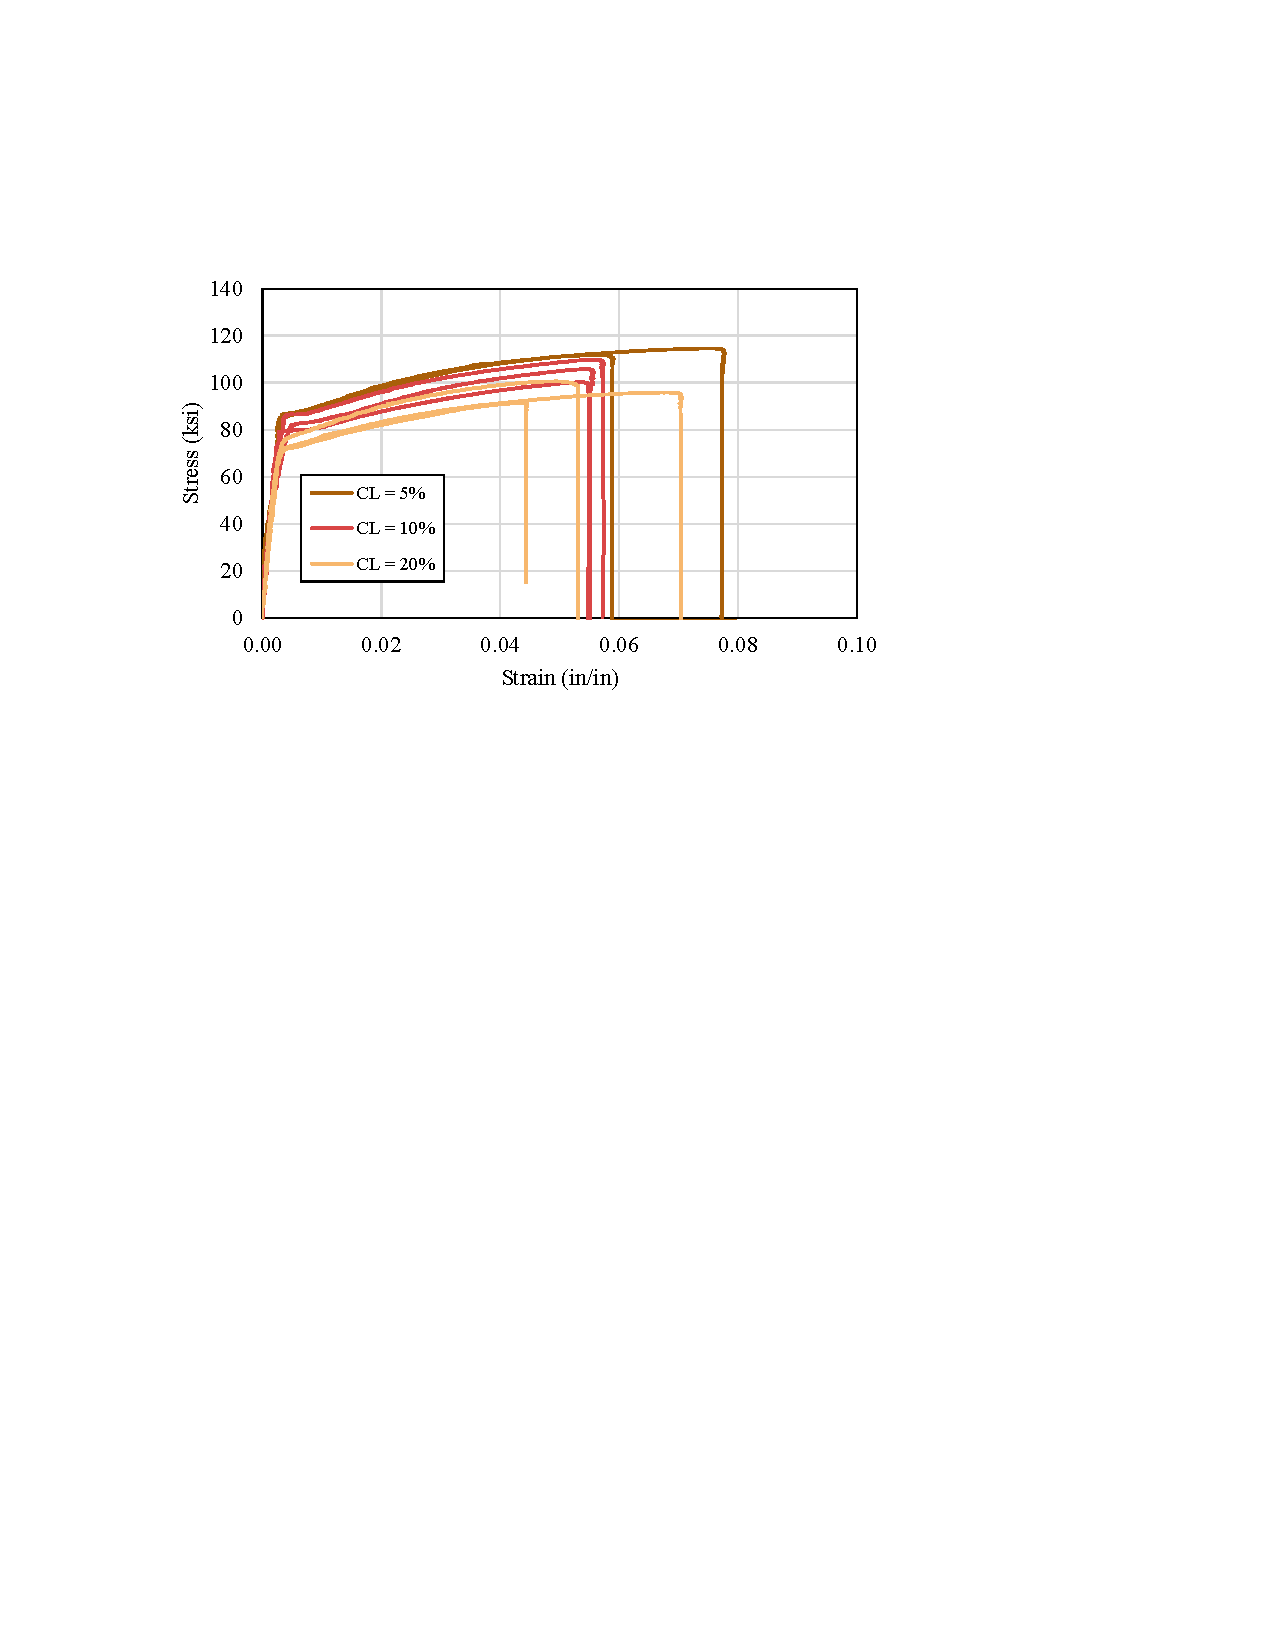
\includegraphics[width=0.7\textwidth]{VAC Thesis 2.0/Chapter-4/figs/TensionTest_results_1.pdf}
	\caption{Tension test results at different corrosion levels}
	\label{fig:TensionTestResults_StressStrain}
\end{figure}

\subsection{Yield strength as a function of corrosion}
\begin{figure}[htbp]
	\centering
	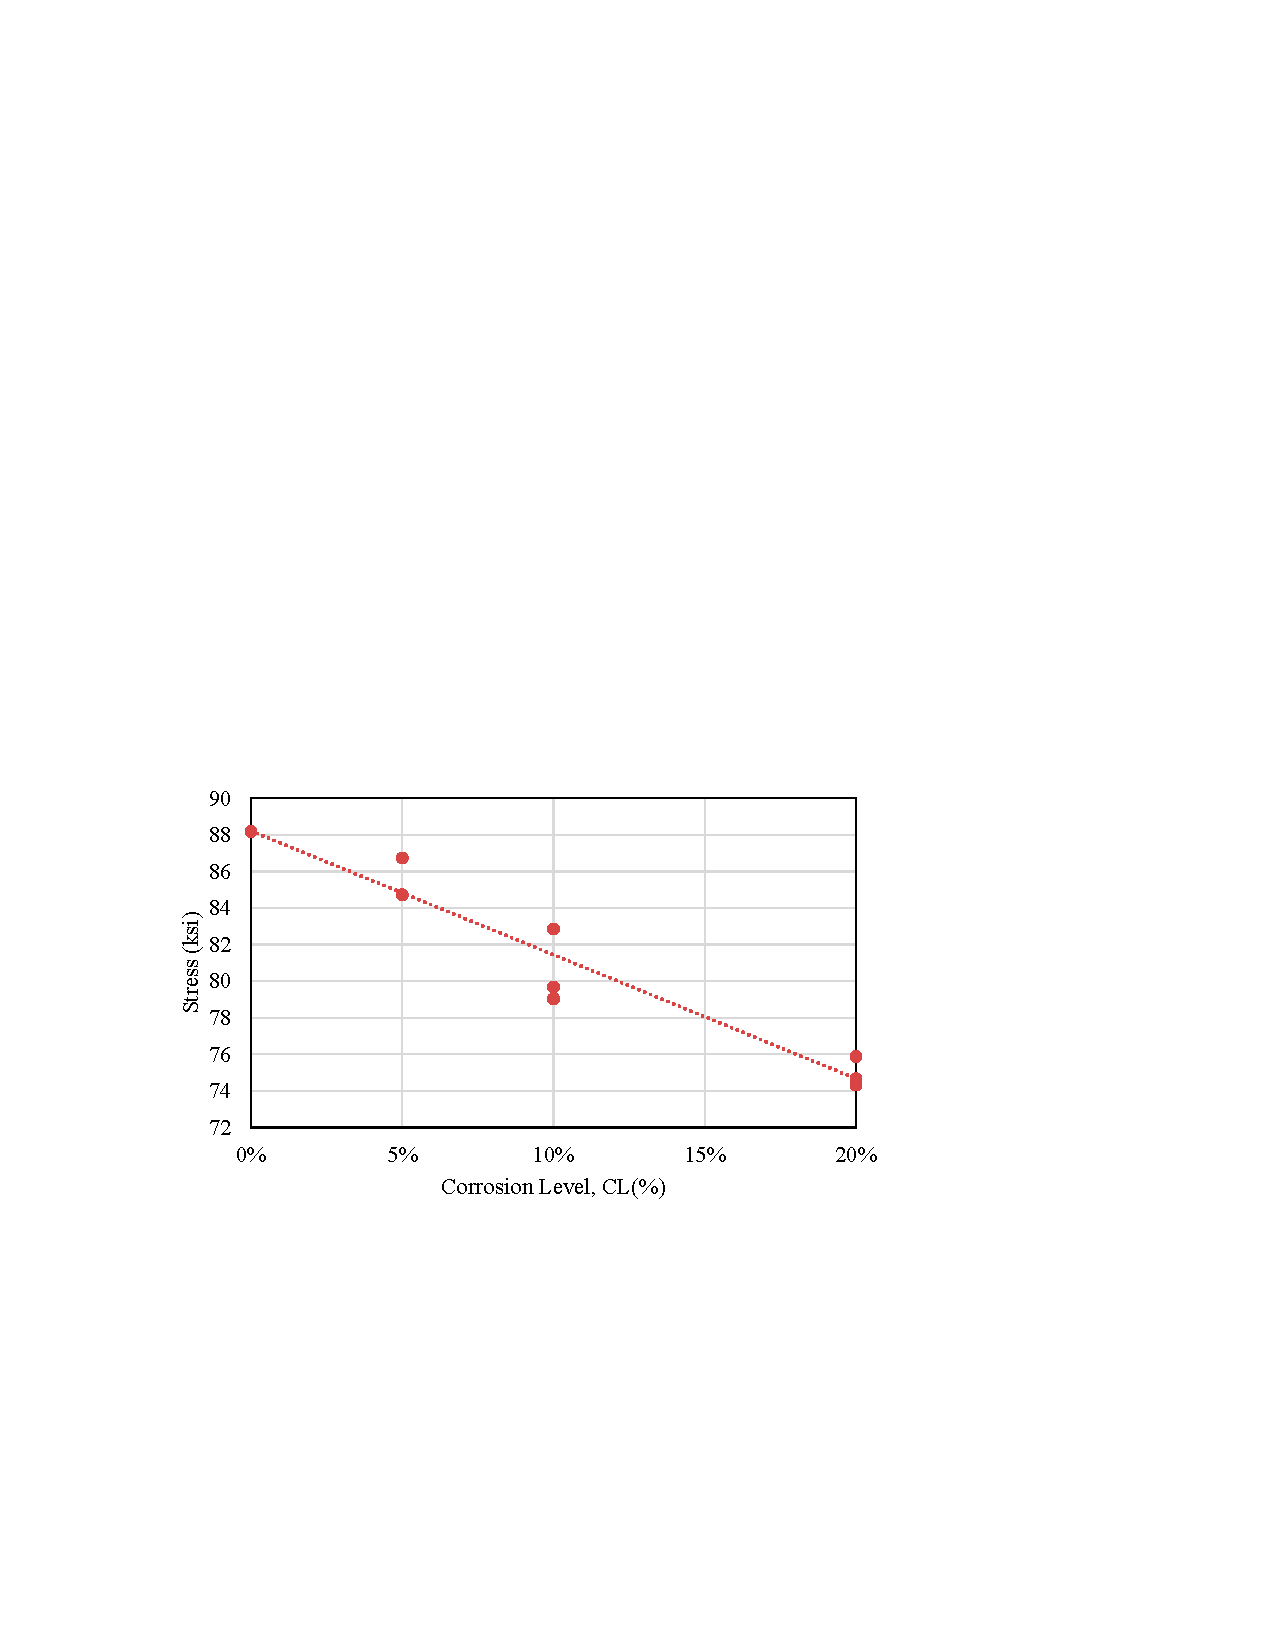
\includegraphics[width=0.7\textwidth]{VAC Thesis 2.0/Chapter-4/figs/TensionTest_results_2.pdf}
	\caption{Yield strength as a function of corrosion level}
	\label{fig:YieldStrength_vs_CL}
\end{figure}
\begin{figure}[htbp]
	\centering
	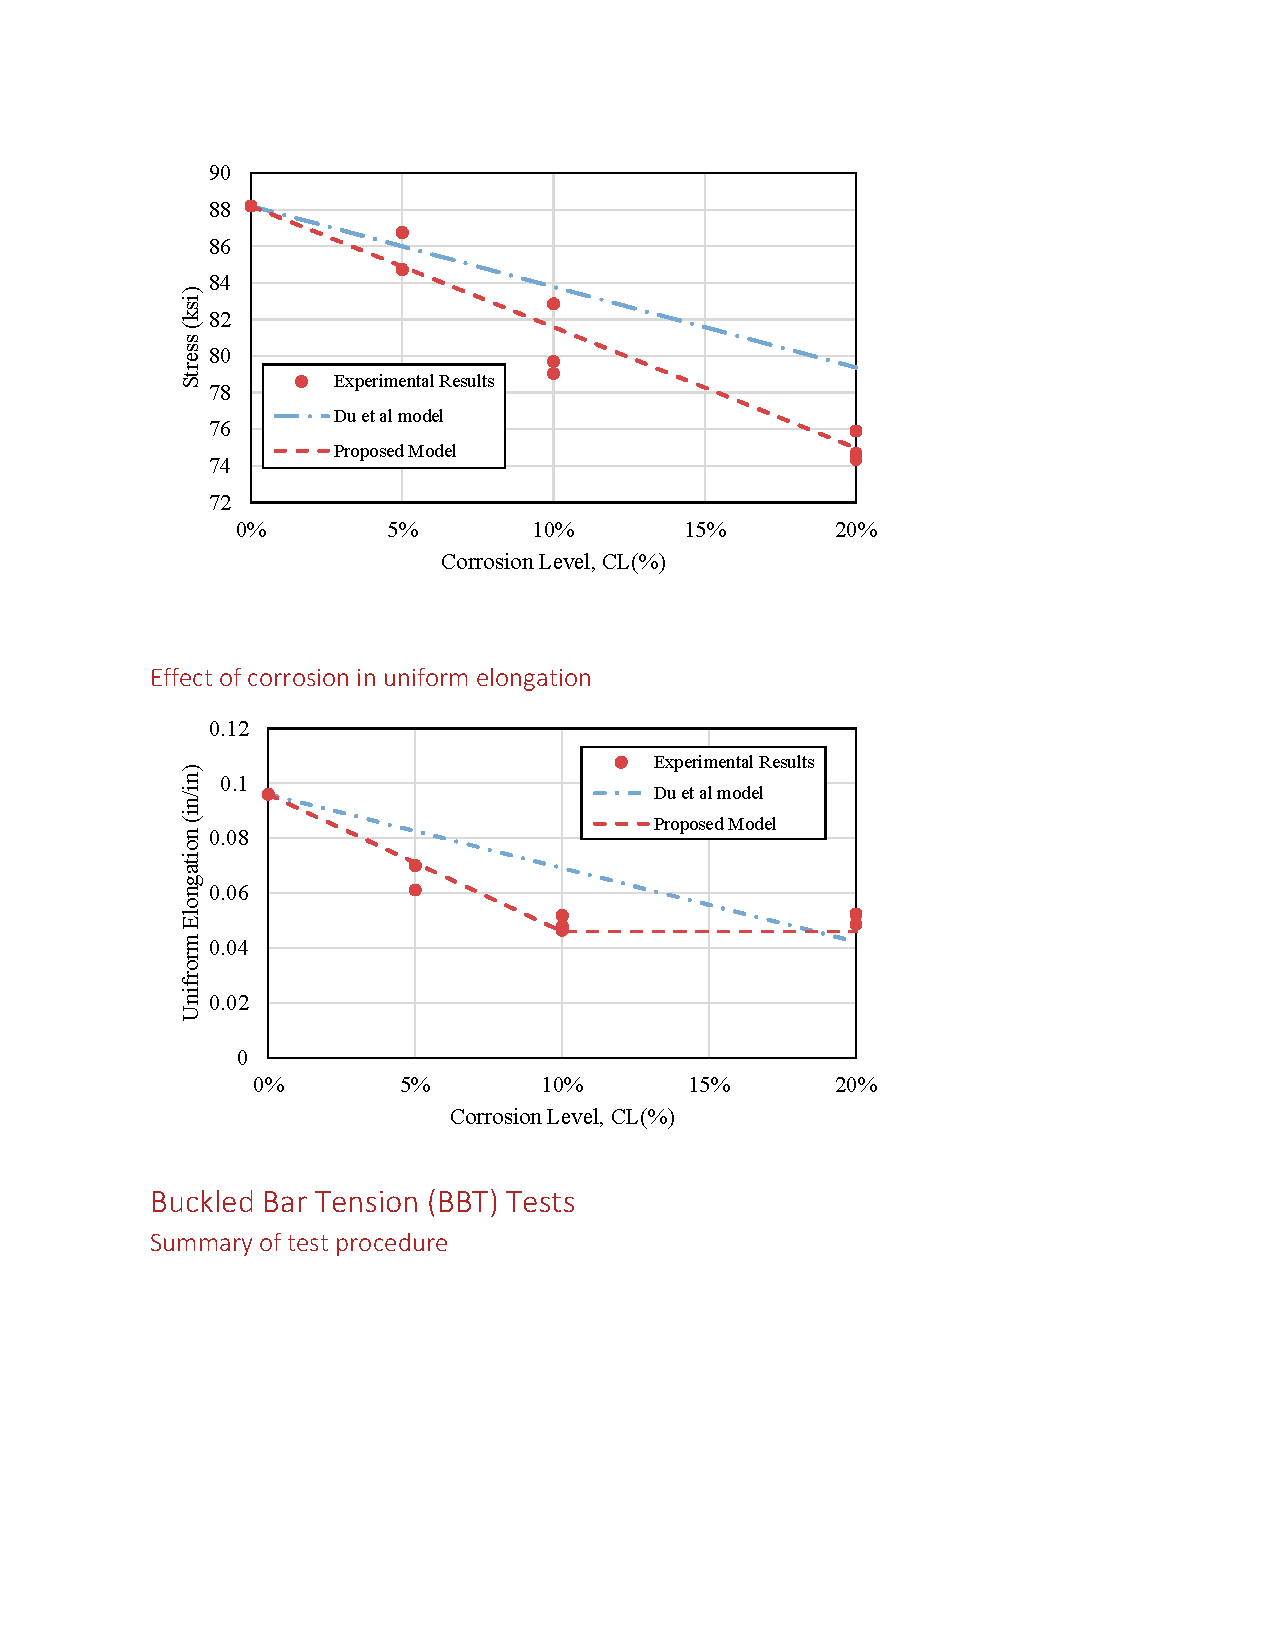
\includegraphics[width=0.7\textwidth]{VAC Thesis 2.0/Chapter-4/figs/TensionTest_results_3_proposedmodel.pdf}
	\caption{Yield strength as a function of corrosion level comparison of proposed model and Du et al model \cite{Du2005}}
	\label{fig:TensionTestResults_StressStrain}
\end{figure}
\subsection{Effect of corrosion in uniform elongation}

\begin{figure}[htbp]
	\centering
	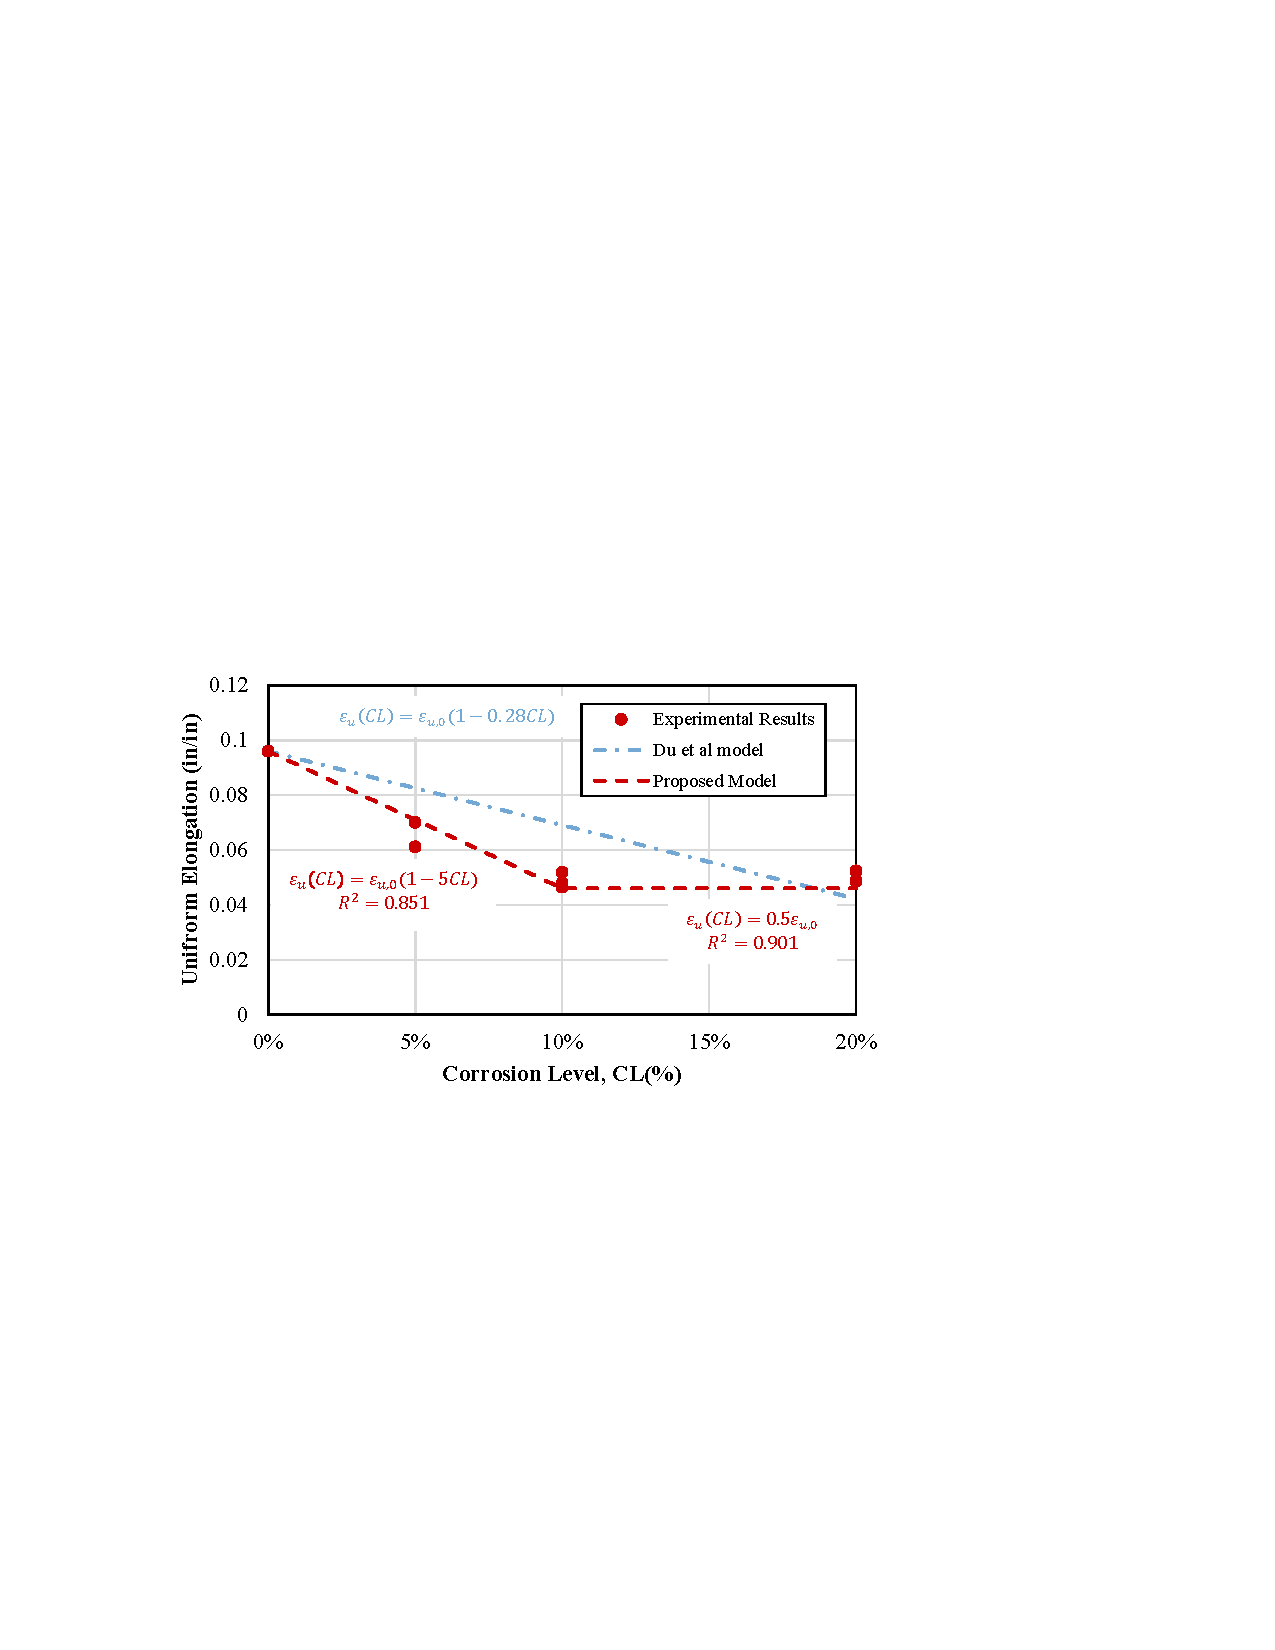
\includegraphics[width=0.7\textwidth]{VAC Thesis 2.0/Chapter-4/figs/TensionTest_results_4_proposedmodel.pdf}
	\caption{Uniform elongation as a function of the corrosion level comparison of proposed model and Du et al model \cite{Du2005}}
	\label{fig:TensionTestResults_StressStrain}
\end{figure}

\section{Buckled Bar Tension (BBT) Tests}

\begin{figure}[htbp]
	\centering
	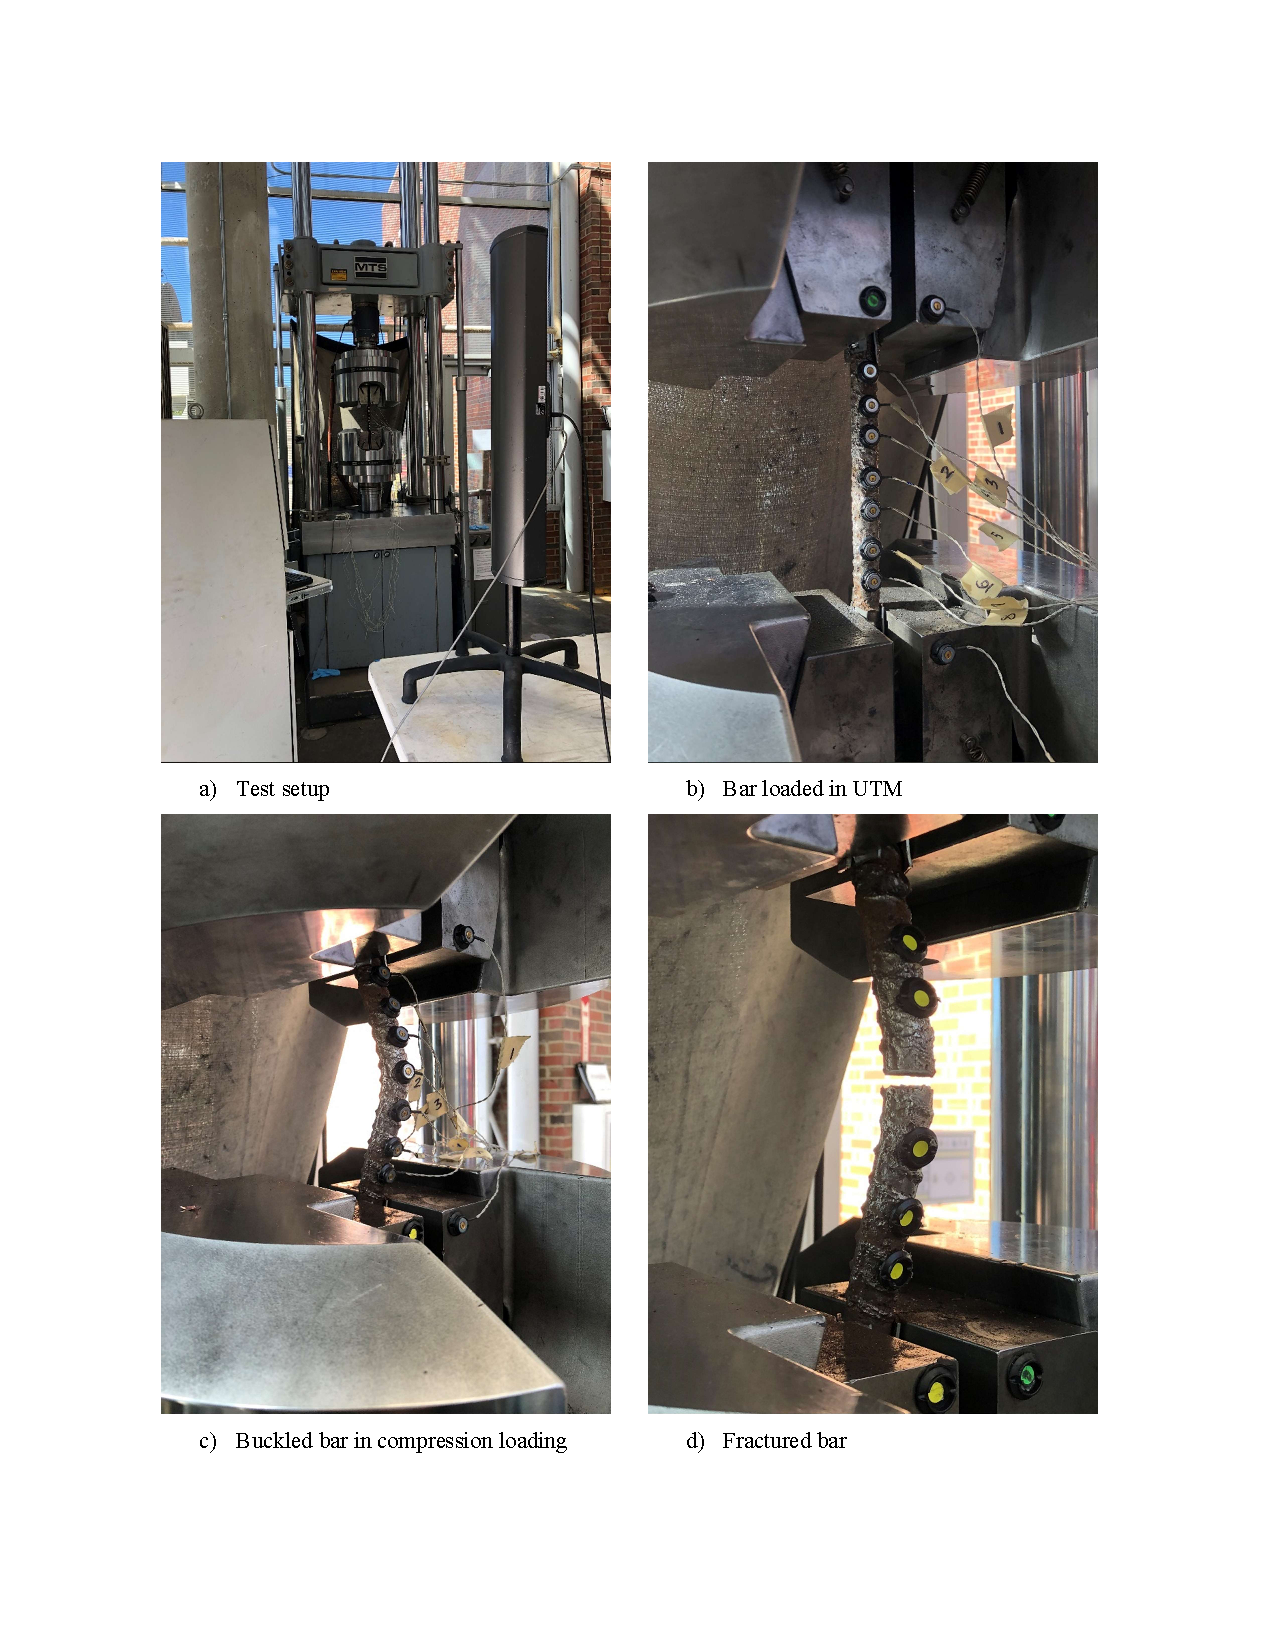
\includegraphics[width=0.7\textwidth]{VAC Thesis 2.0/Chapter-4/figs/BBT Procedure.pdf}
	\caption{General procedure of buckled bar tension (BBT) test}
	\label{fig:BBT_Test_Summary}
\end{figure}

\begin{figure}[htbp]
	\centering
	\includegraphics[width=0.7\textwidth]{VAC Thesis 2.0/Chapter-4/figs/BBT}
	\caption{General procedure of buckled bar tension (BBT) test}
	\label{fig:BBT_Test_Summary}
\end{figure}

\subsection{Effect of corrosion in Critical Bending Strain}
\begin{figure}[htbp]
	\centering
	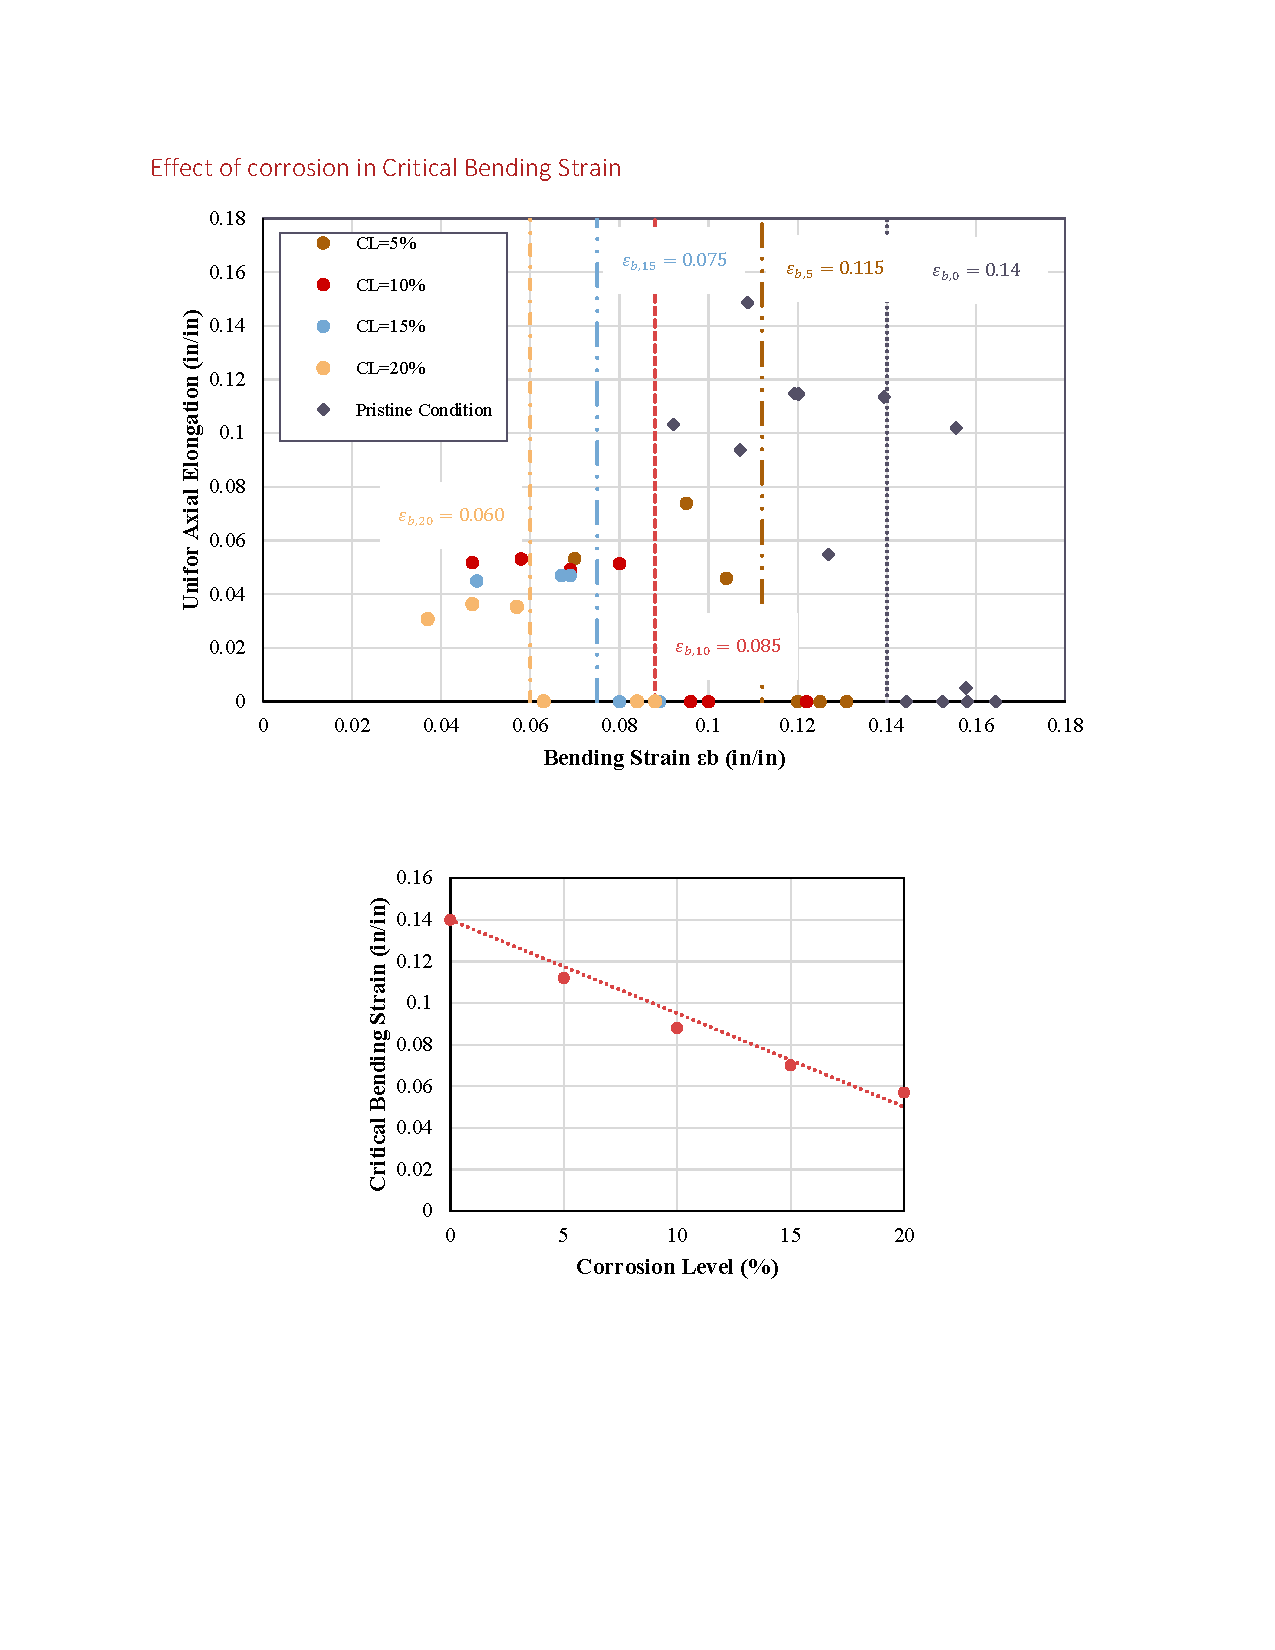
\includegraphics[width=0.7\textwidth]{VAC Thesis 2.0/Chapter-4/figs/BBT_results_.pdf}
	\caption{Bending strain at different corrosion levels}
	\label{fig:BBT_strains}
\end{figure}
\begin{figure}[htbp]
	\centering
	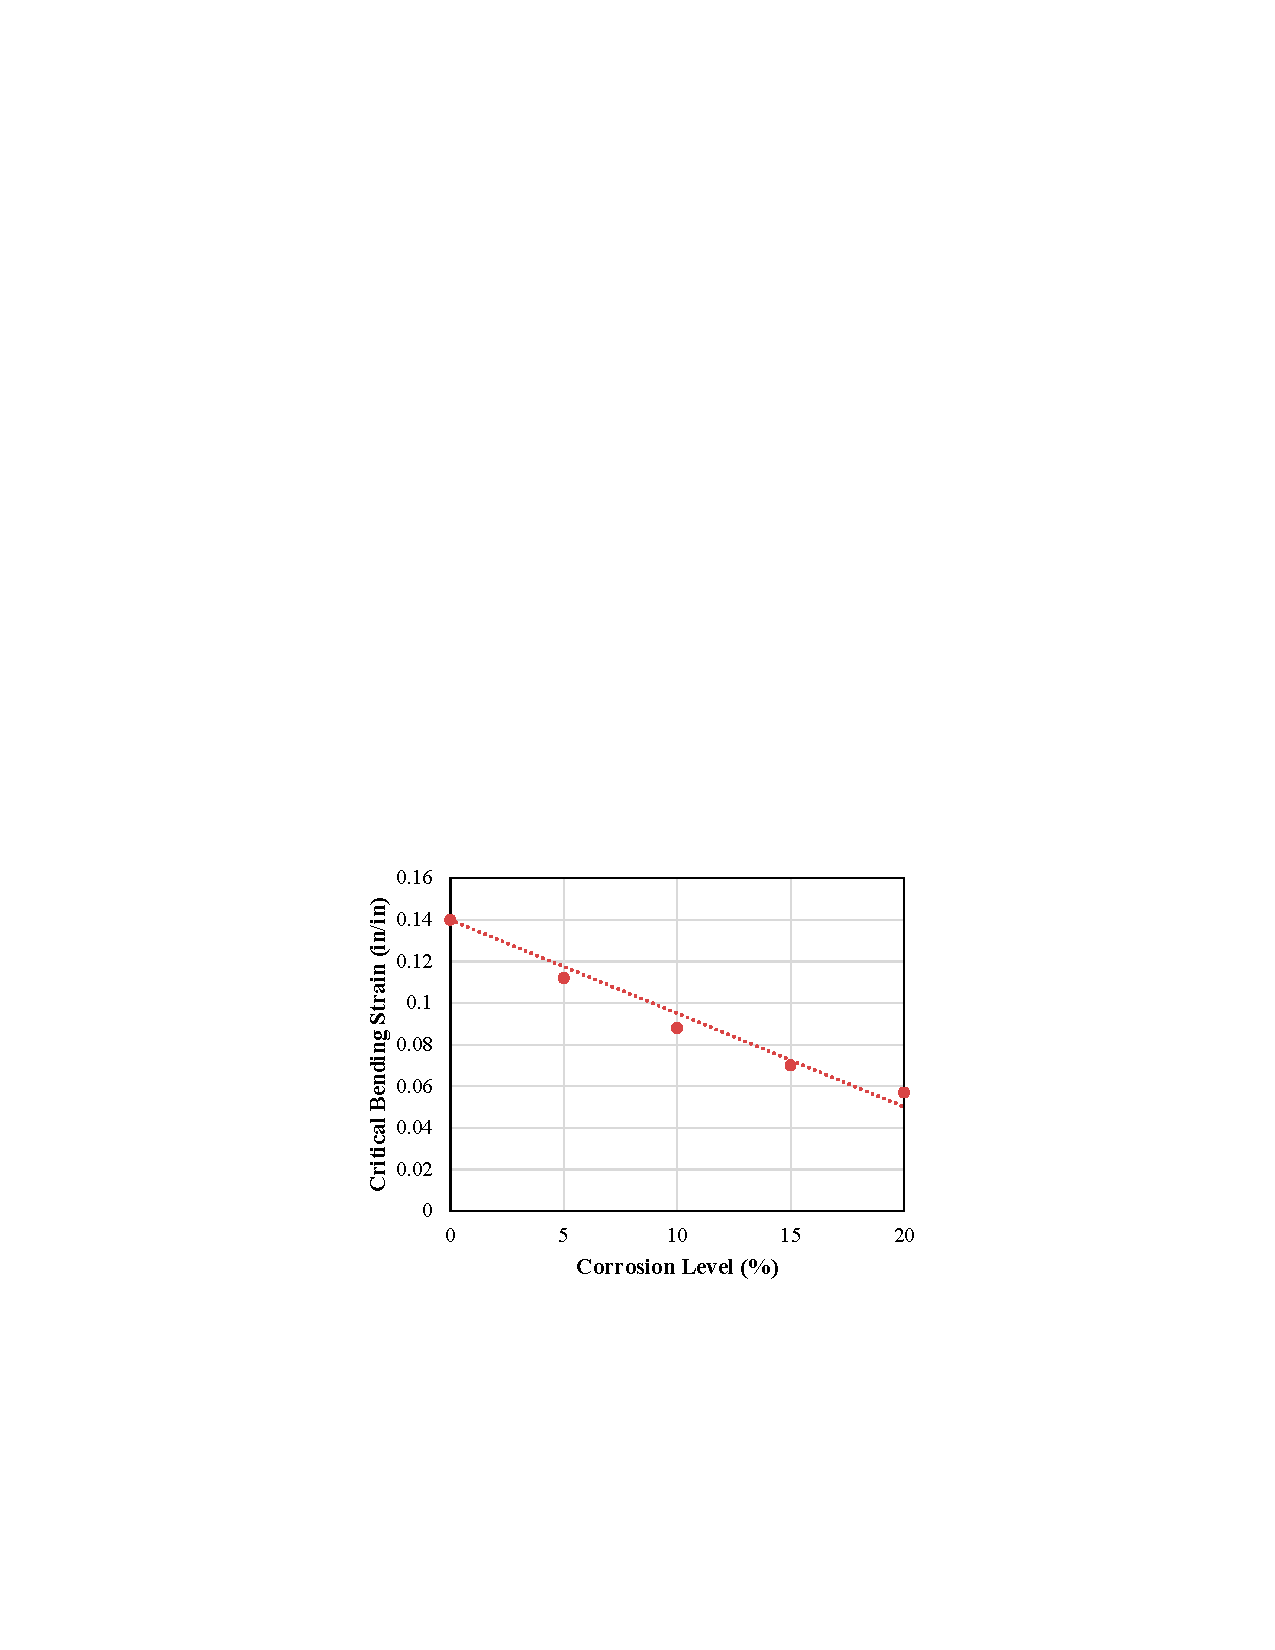
\includegraphics[width=0.7\textwidth]{VAC Thesis 2.0/Chapter-4/figs/BBT_results_summary.pdf}
	\caption{Maximum bending strain as a function of corrosion level}
	\label{fig:eb_vs_CL}
\end{figure}
\subsection{Effect of corrosion at the micro-structural level}
\textbf{Fractography}
\begin{figure}[htbp]
	\centering
	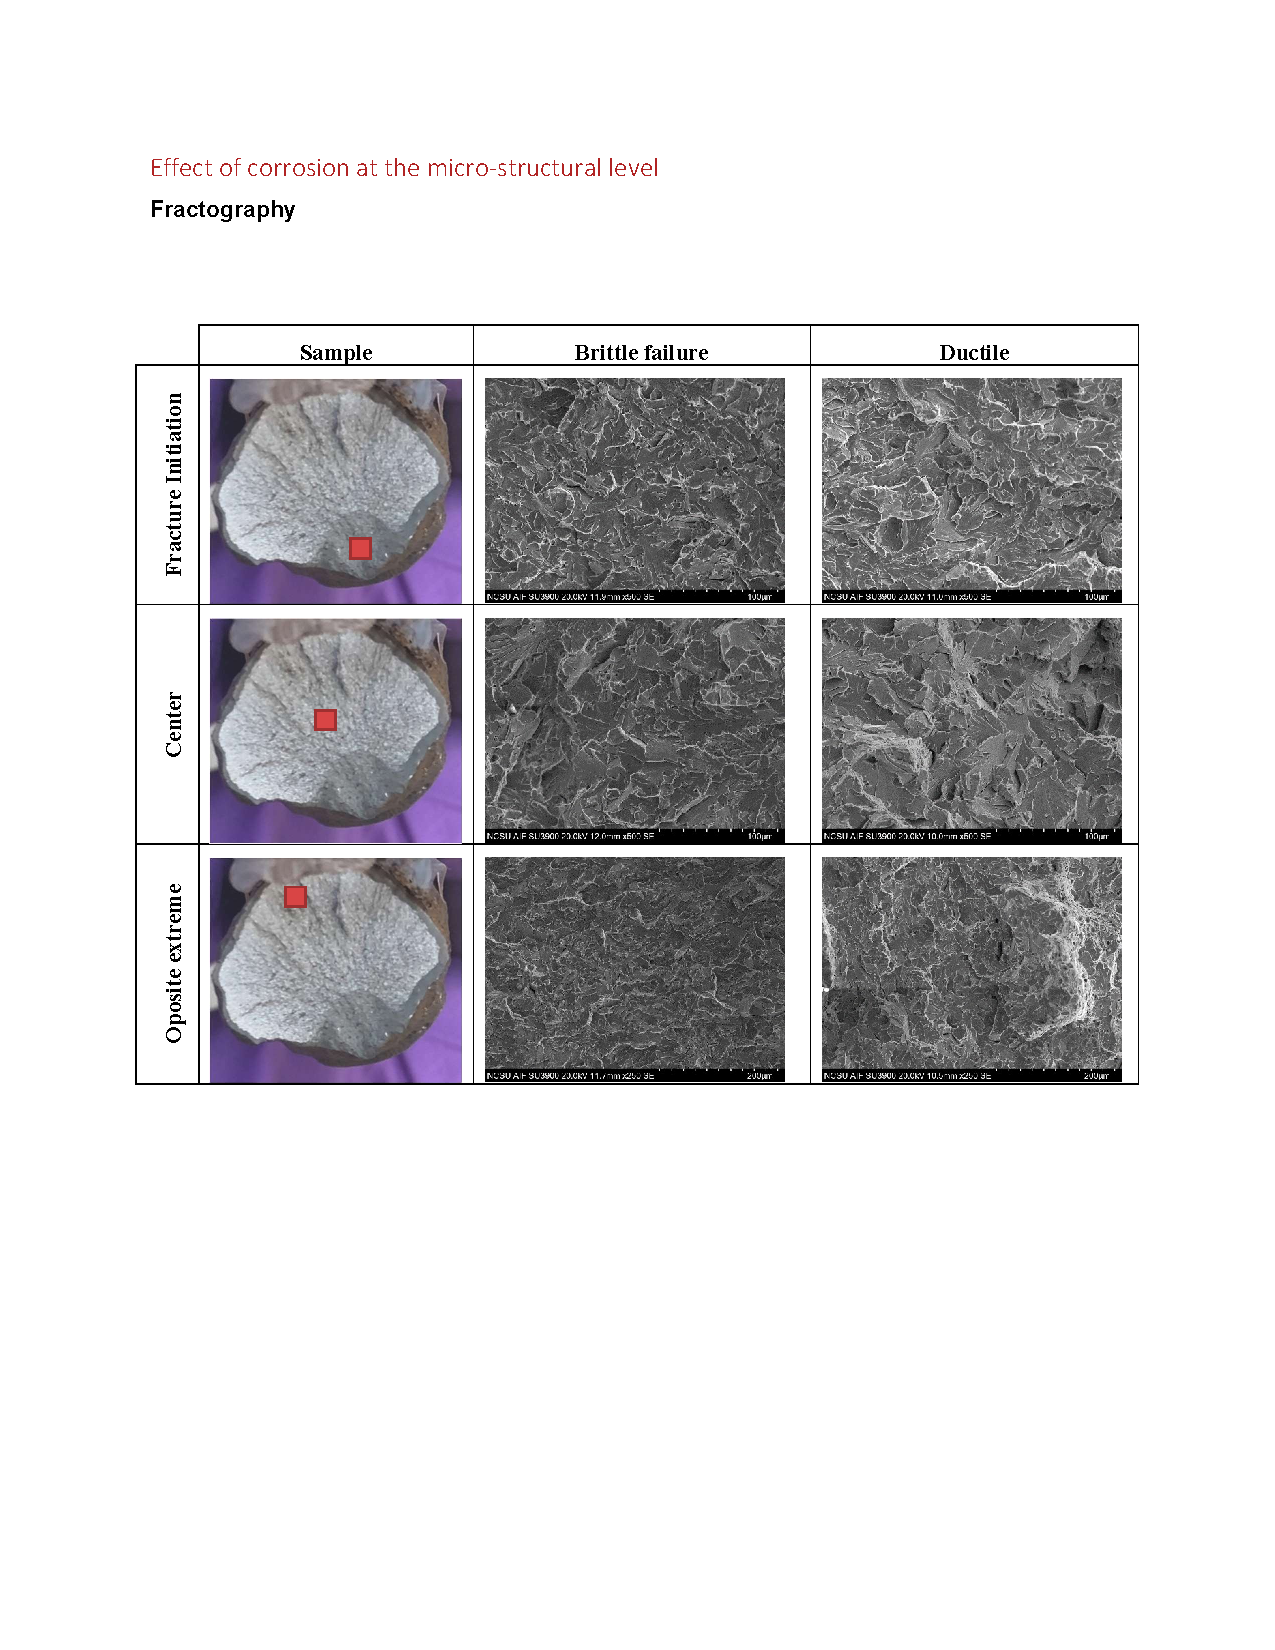
\includegraphics[width=1\textwidth]{VAC Thesis 2.0/Chapter-4/figs/BBT_fractography.pdf}
	\caption{SEM observations for brittle and ductile failure at different positions of the fracture surface}
	\label{fig:FractureSurfaces}
\end{figure}
\begin{figure}[htbp]
	\centering
	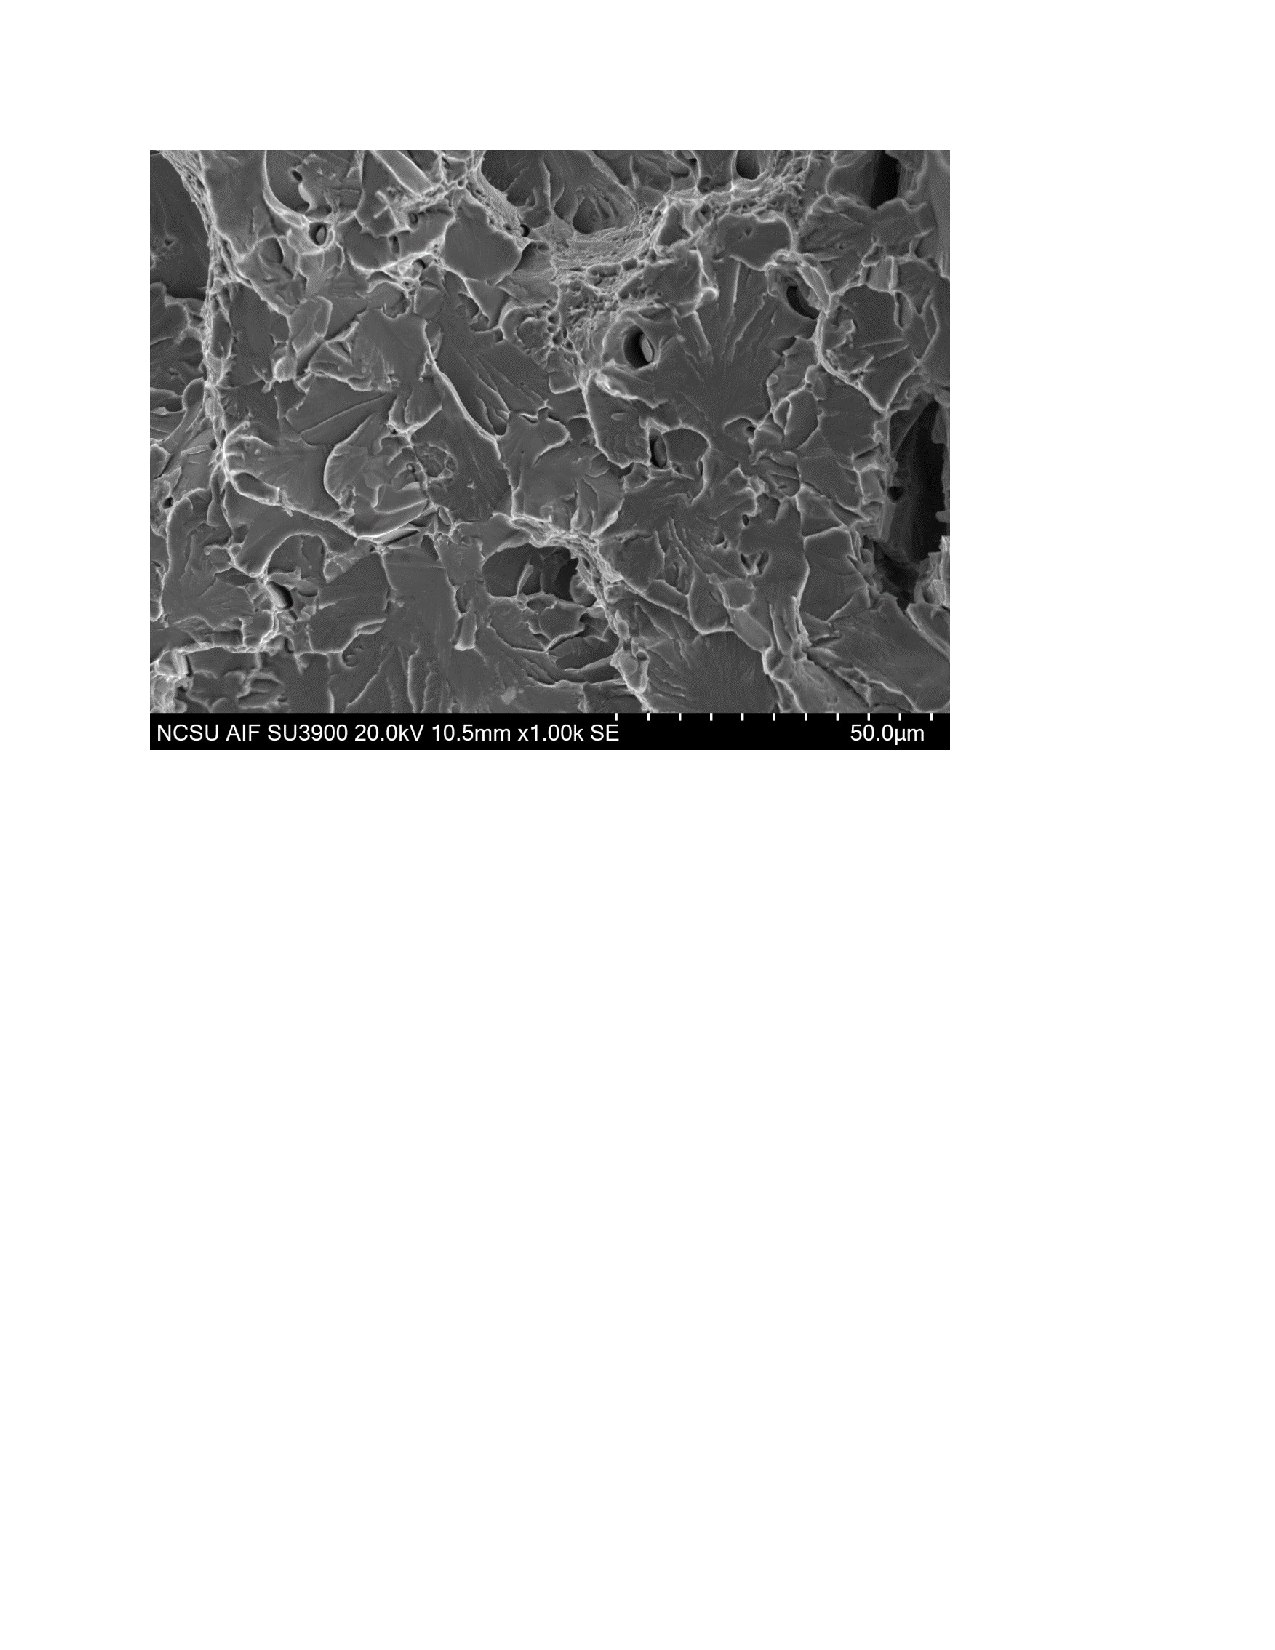
\includegraphics[width=0.7\textwidth]{VAC Thesis 2.0/Chapter-4/figs/BBT_RiverFeatures.pdf}
	\caption{SEM cyclic loading features in fracture surface at 500x magnification}
	\label{fig:RiverFeatures}
\end{figure}
\textbf{Spectrum analysis}
\begin{figure}[htbp]
	\centering
	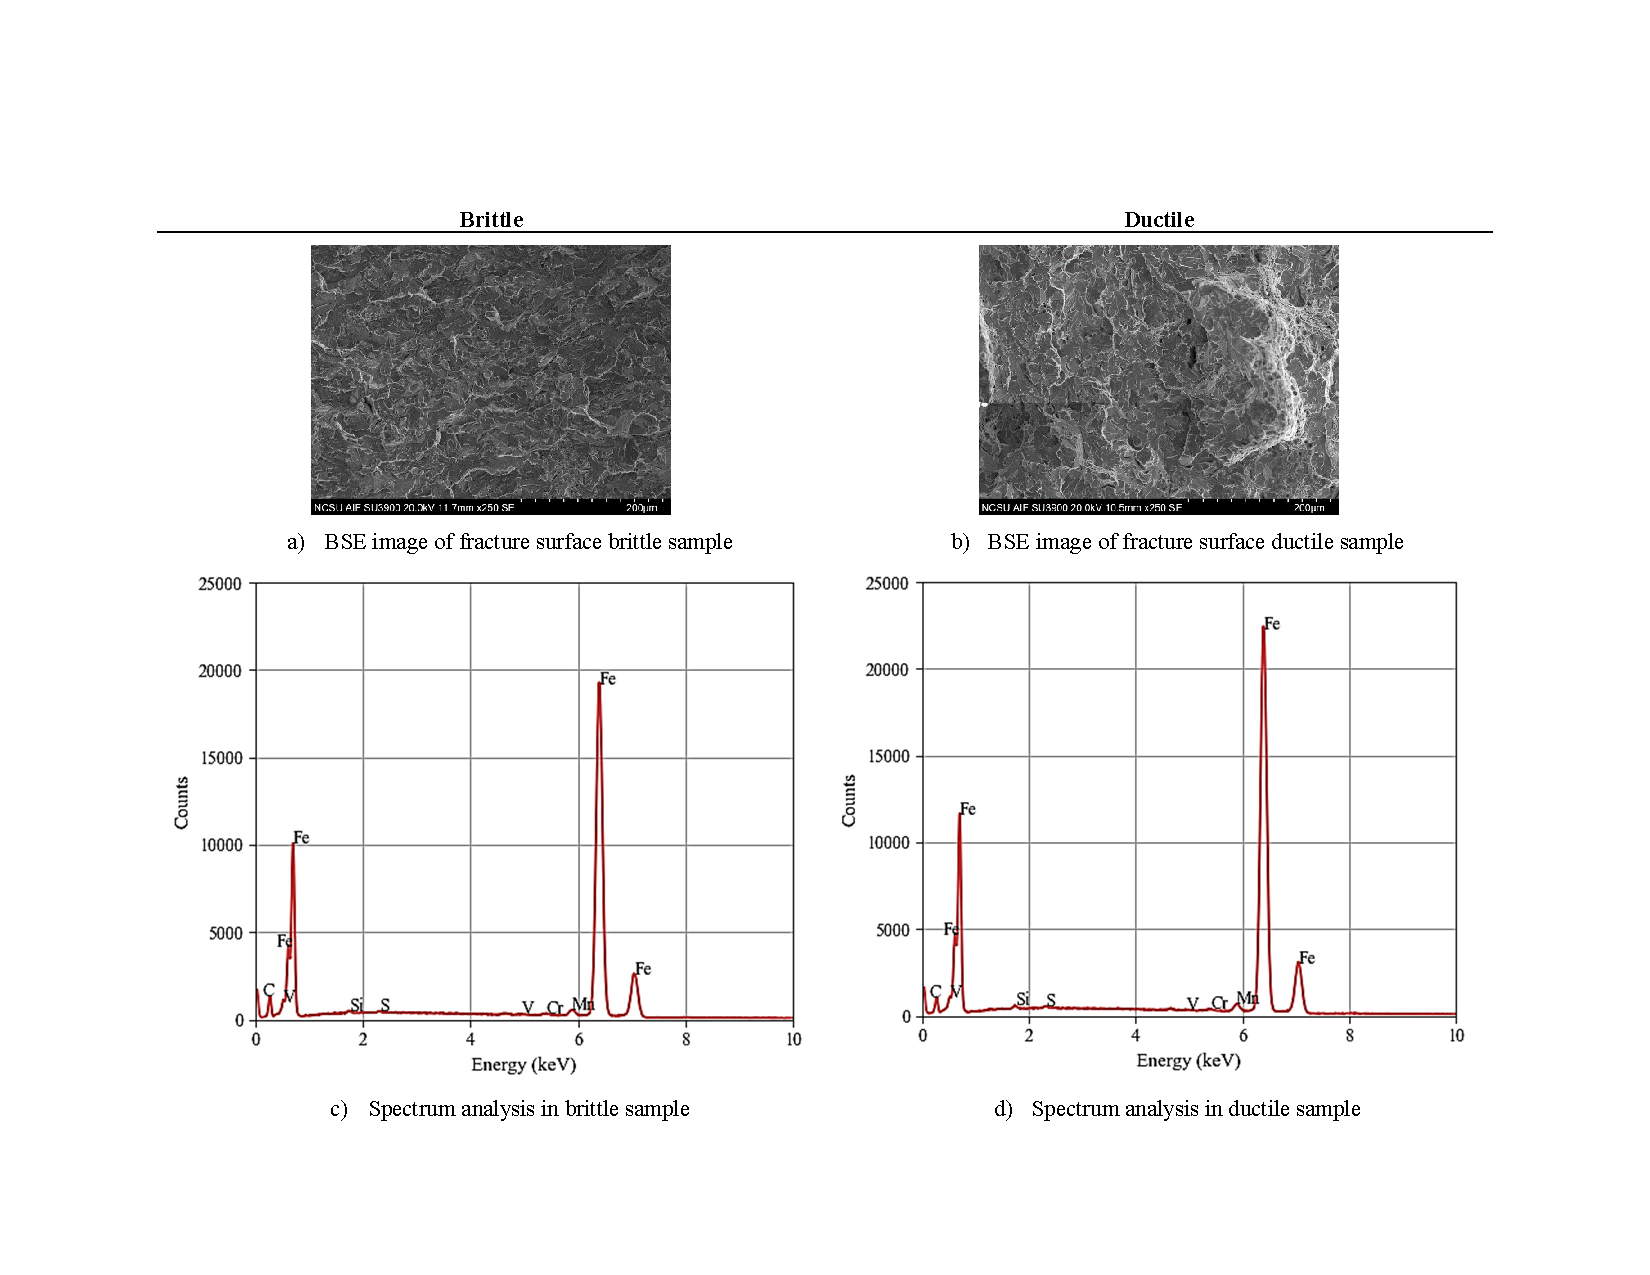
\includegraphics[width=0.9\textwidth]{VAC Thesis 2.0/Chapter-4/figs/BBT_SpectrumAnalysis.pdf}
	\caption{Spectrum analysis of Back Scatter Electrons of fracture surface for brittle and ductile failures}
	\label{fig:SpectrumAnalysis}
\end{figure}
\subsection{Effect of geometry imperfections}